\section{Computer Simulations}  \label{comp_simulation}
\begin{figure}[H]
    \centering
    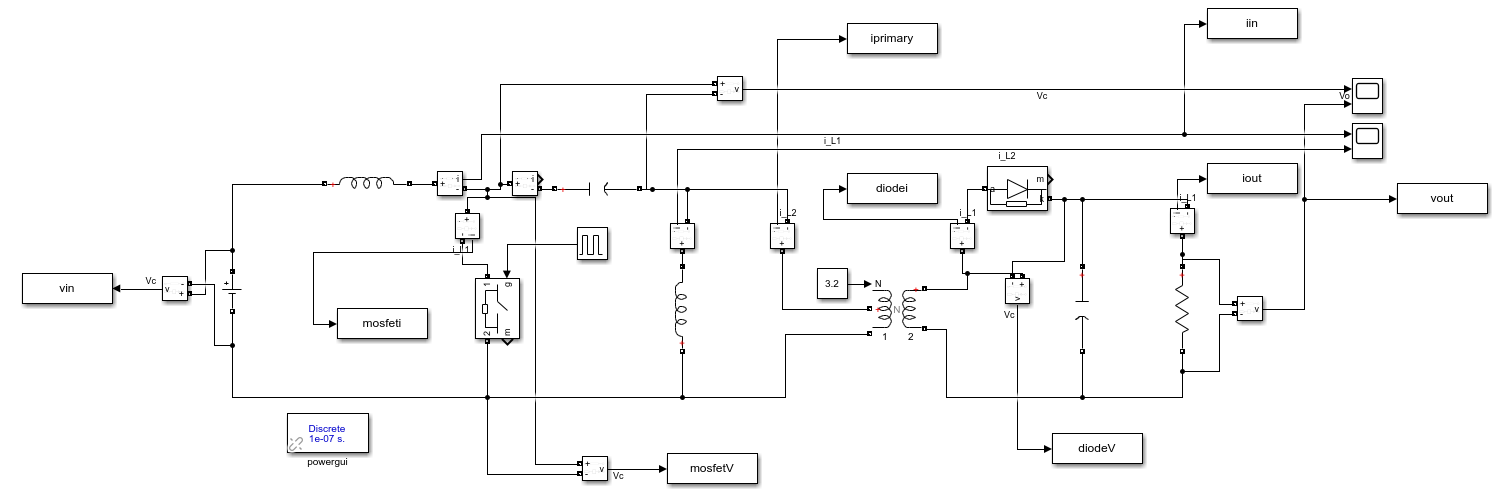
\includegraphics[width=\textwidth]{Figures/mat_cirr.png}
    \caption{Simulink simulation circuit for ideal case.}
    \label{fig:simulink}
\end{figure}
\begin{figure}[H]
    \centering
    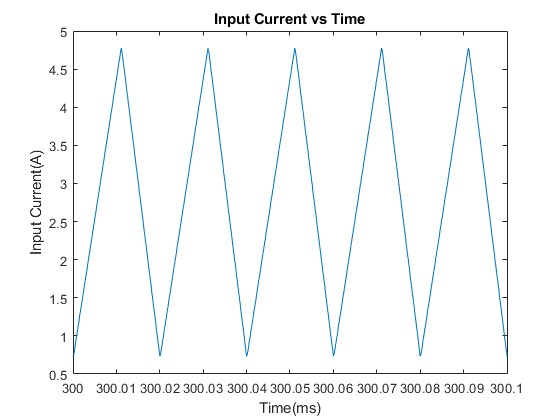
\includegraphics[width=0.6\textwidth]{Figures/mat_iin.jpg}
    \caption{$I_{in}$ versus time graph ideal case.}
    \label{fig:mat_i_in}
\end{figure}
\begin{figure}[H]
    \centering
    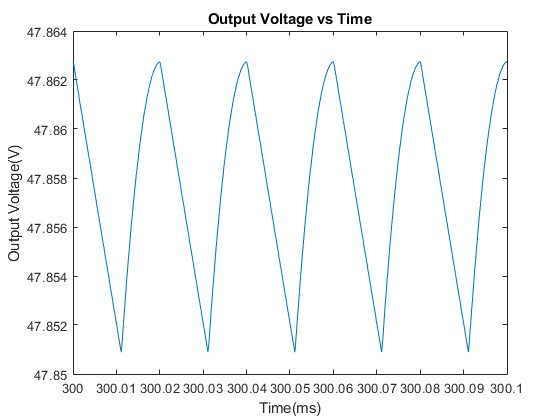
\includegraphics[width=0.6\textwidth]{Figures/mat_vout.jpg}
    \caption{$V_{out}$ versus time graph ideal case.}
    \label{fig:mat_v_out}
\end{figure}
\begin{figure}[H]
    \centering
    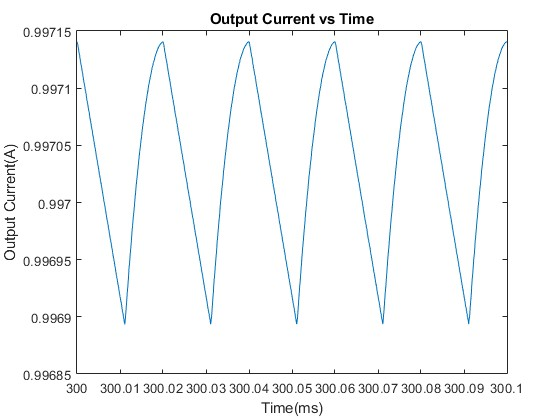
\includegraphics[width=0.6\textwidth]{Figures/mat_iout.jpg}
    \caption{$I_{out}$ versus time graph ideal case.}
    \label{fig:mat_i_out}
\end{figure}
\begin{figure}[H]
    \centering
    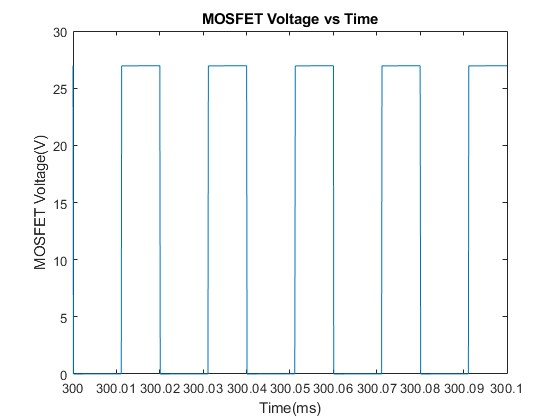
\includegraphics[width=0.6\textwidth]{Figures/mat_mos_volt.jpg}
    \caption{MOSFET voltage versus time graph ideal case.}
    \label{fig:mat_v_sw}
\end{figure}
\begin{figure}[H]
    \centering
    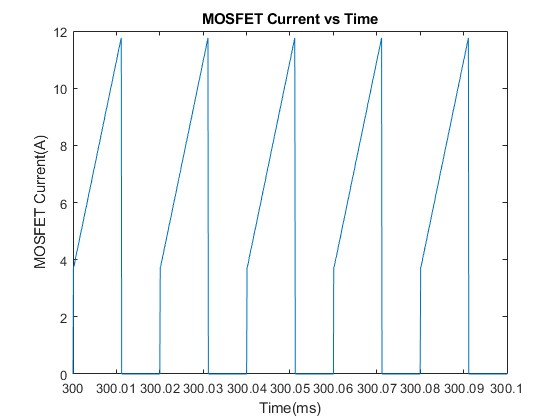
\includegraphics[width=0.6\textwidth]{Figures/mat_mos_curr.jpg}
    \caption{MOSFET current versus time graph ideal case.}
    \label{fig:mat_i_sw}
\end{figure}
\begin{figure}[H]
    \centering
    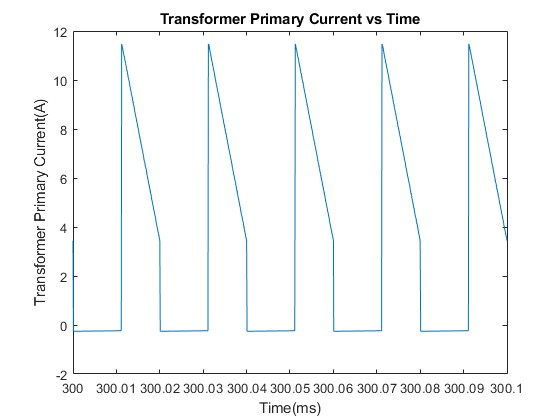
\includegraphics[width=0.6\textwidth]{Figures/mat_prim_current.jpg}
    \caption{Current on the transformer primary winding versus time ideal case.}
    \label{fig:mat_lm}
\end{figure}
\begin{figure}[H]
    \centering
    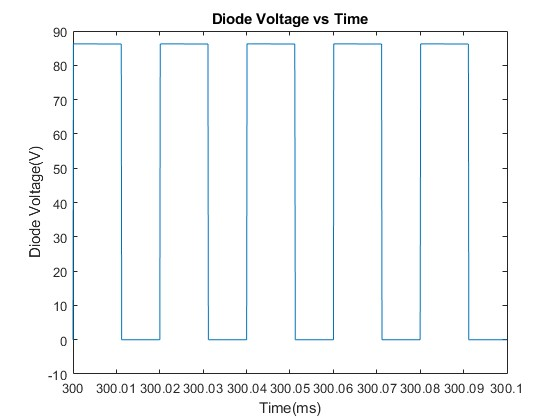
\includegraphics[width=0.6\textwidth]{Figures/mat_diode_volt.jpg}
    \caption{Diode voltage versus time graph ideal case.}
    \label{fig:mat_v_d}
\end{figure}
\begin{figure}[H]
    \centering
    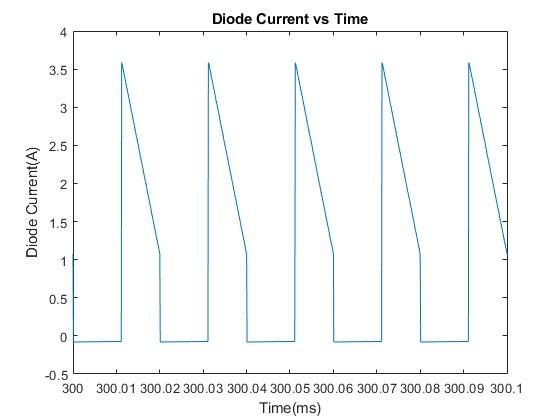
\includegraphics[width=0.6\textwidth]{Figures/mat_diode_current.jpg}
    \caption{Diode current versus time graph ideal case.}
    \label{fig:mat_i_d}
\end{figure}
\begin{figure}[H]
    \centering
    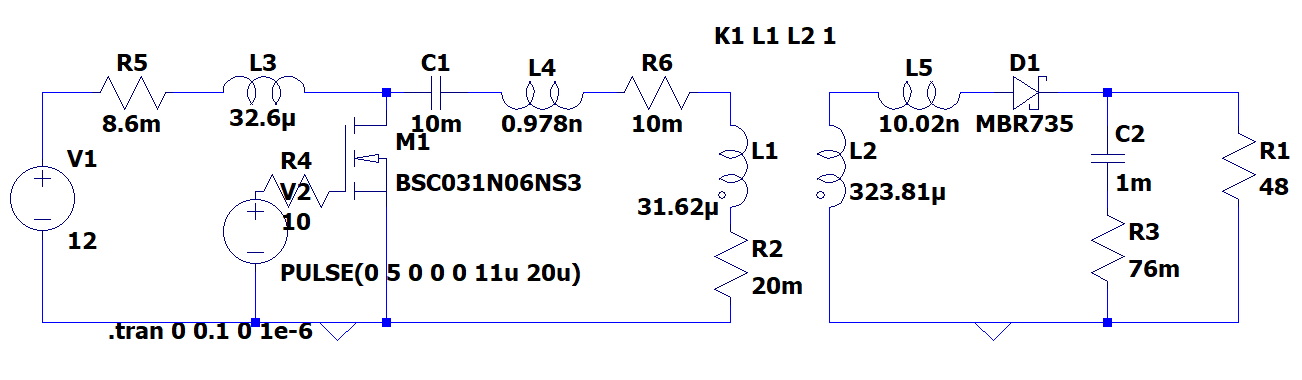
\includegraphics[width=\textwidth]{Figures/spice_circuit.png}
    \caption{LTSpice Circuit Diagram used for simulating the circuit with parasitic.}
    \label{fig:spice}
\end{figure}
\begin{figure}[H]
    \centering
    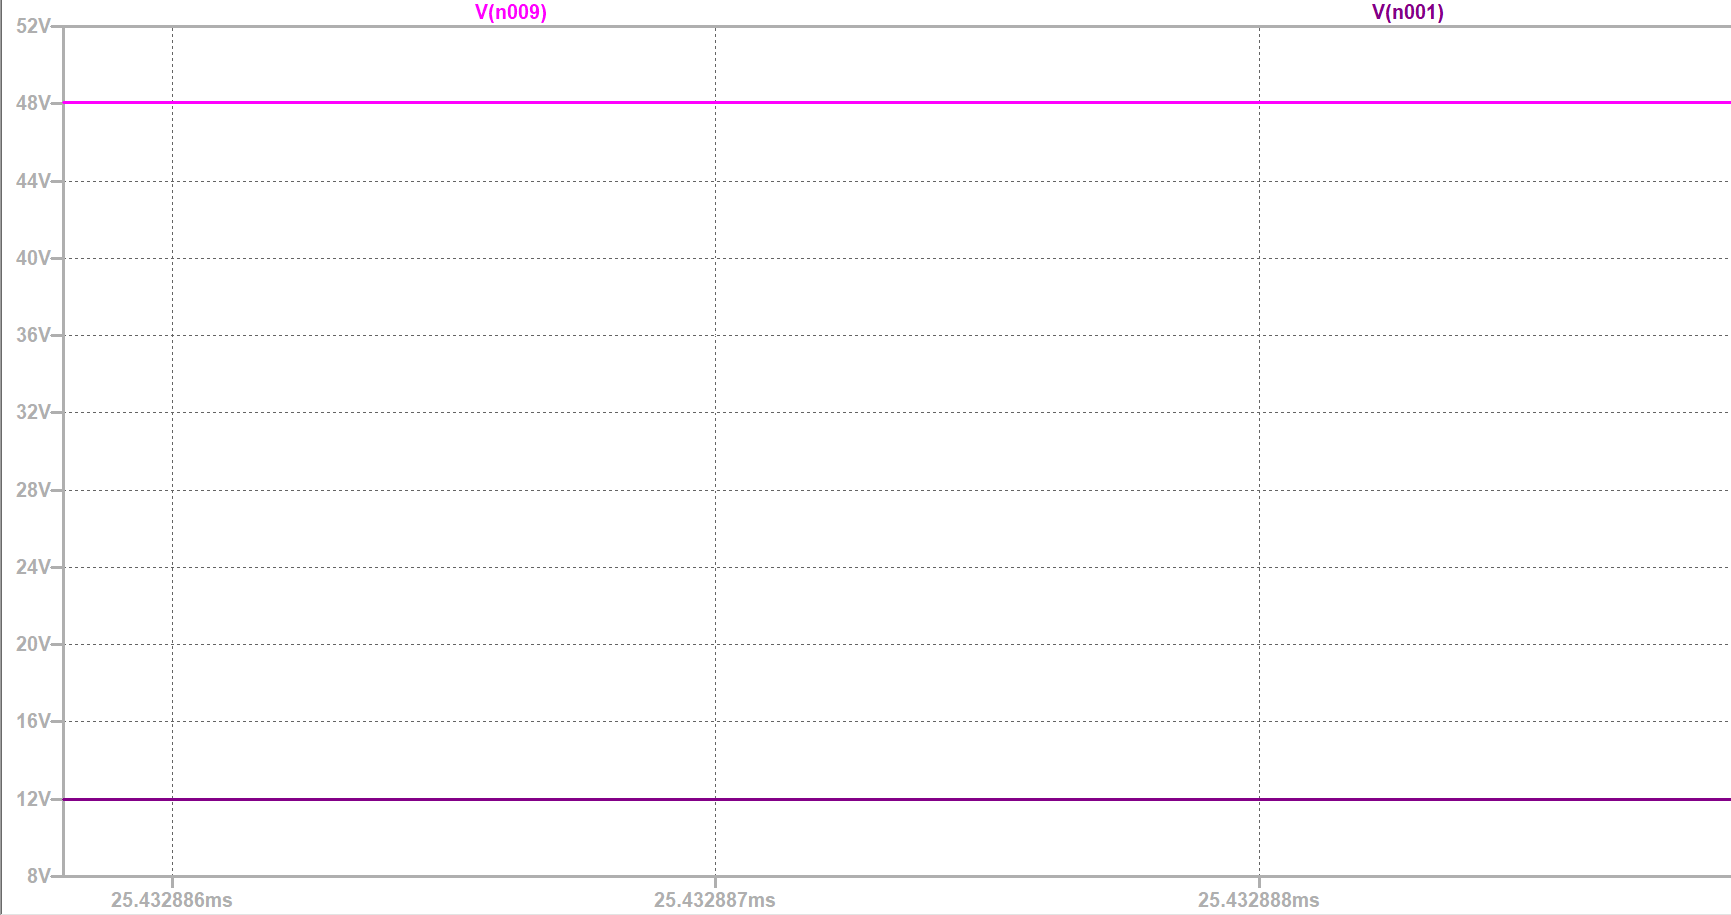
\includegraphics[width=0.6\textwidth]{Figures/vout-vin.png}
    \caption{$V_{out}$ and $V_{in}$ with parasitic included.}
    \label{fig:v_out_v_in}
\end{figure}
\begin{figure}[H]
    \centering
    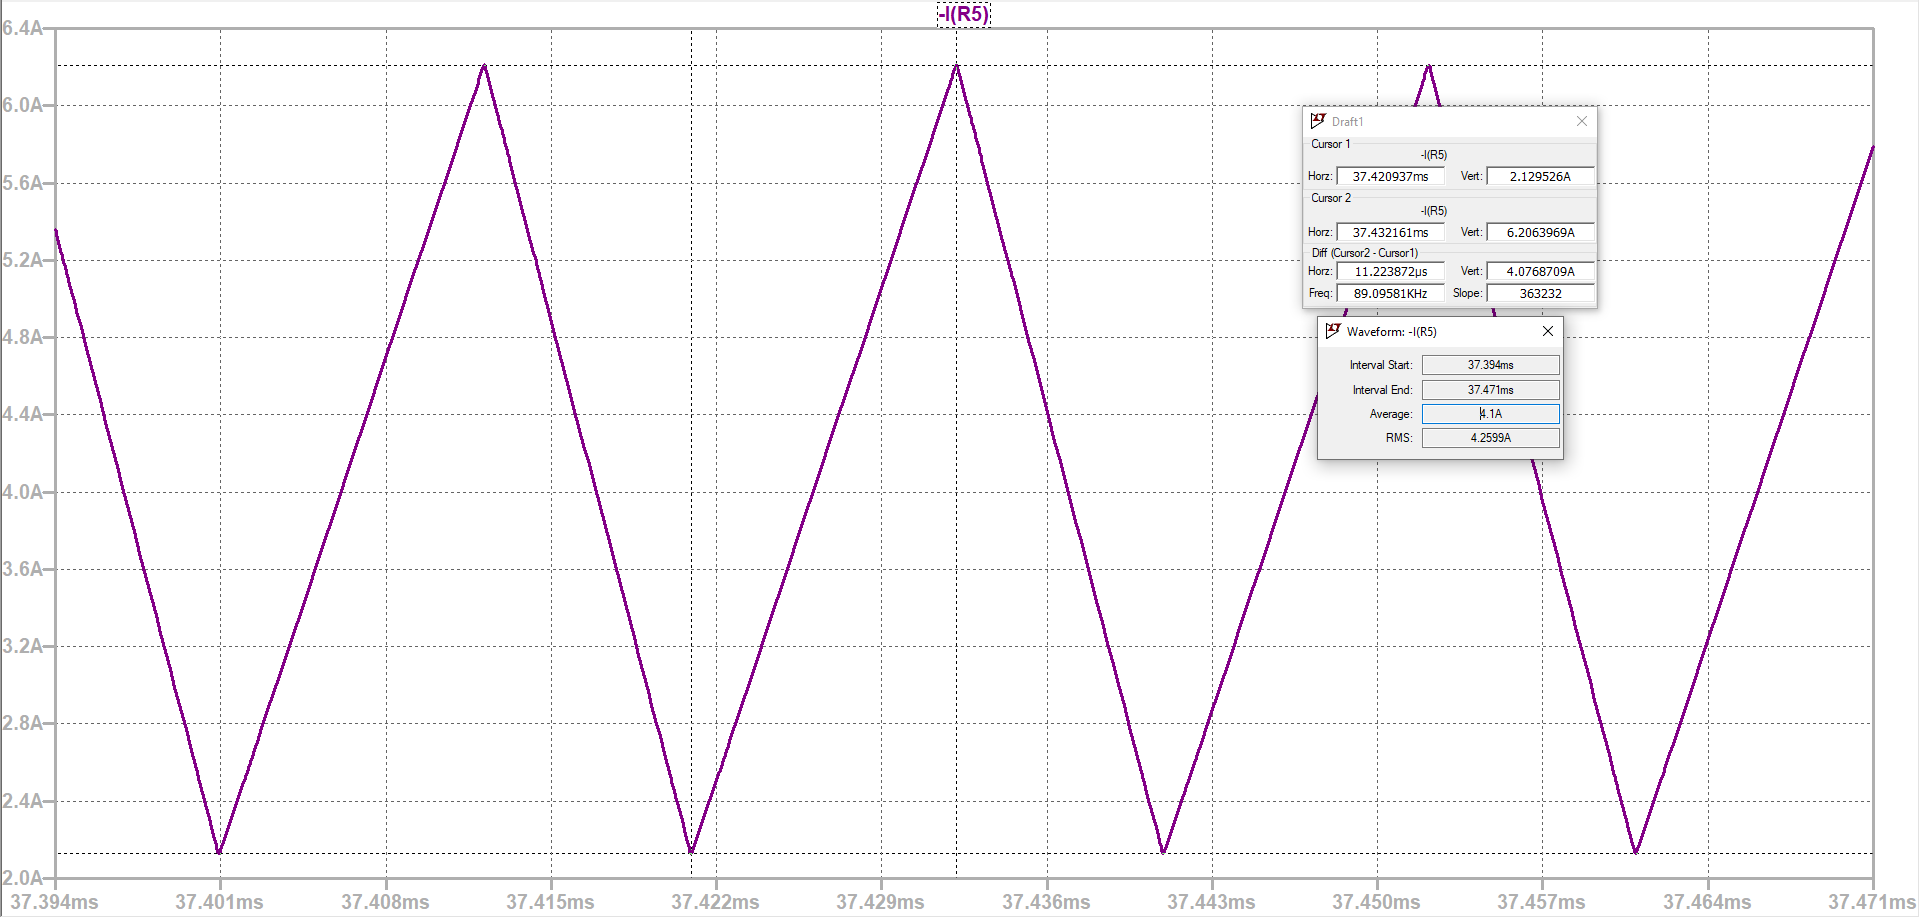
\includegraphics[width=0.6\textwidth]{Figures/in-av-ripple.png}
    \caption{$I_{in}$ waveform with parasitic included.}
    \label{fig:i_in}
\end{figure}
\begin{figure}[H]
    \centering
    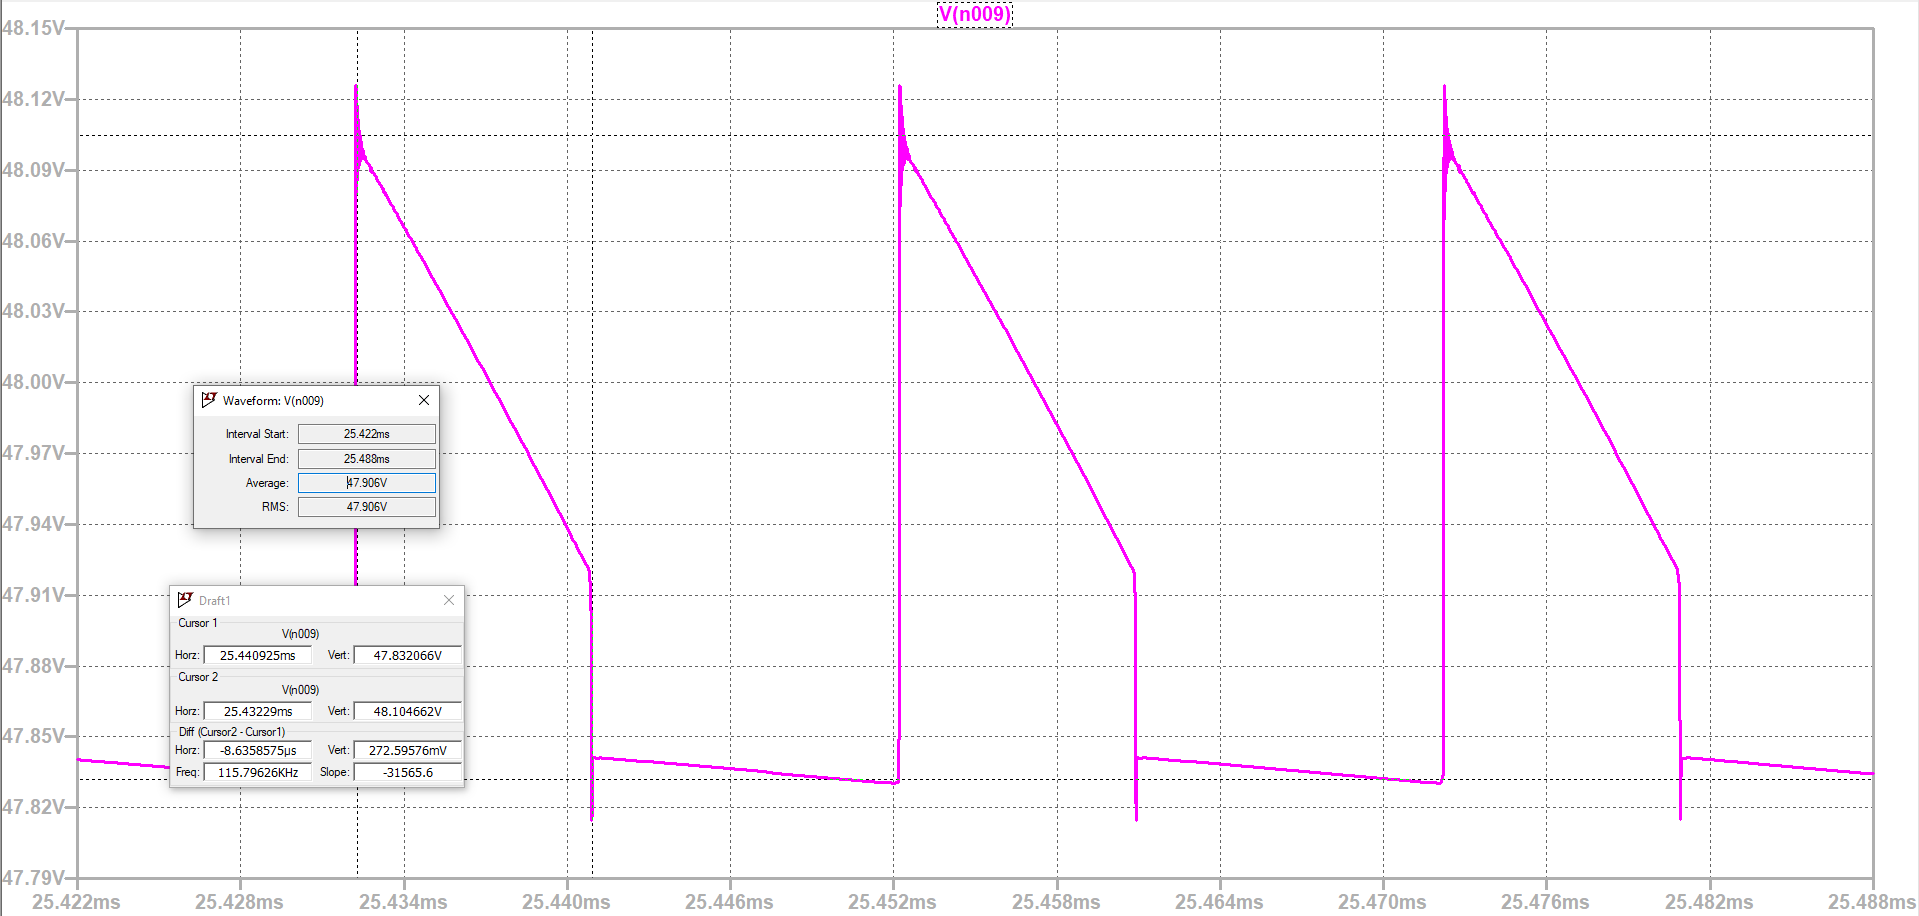
\includegraphics[width=0.6\textwidth]{Figures/vout-av-ripple.png}
    \caption{$V_{out}$ waveform with parasitic included.}
    \label{fig:v_out}
\end{figure}
\begin{figure}[H]
    \centering
    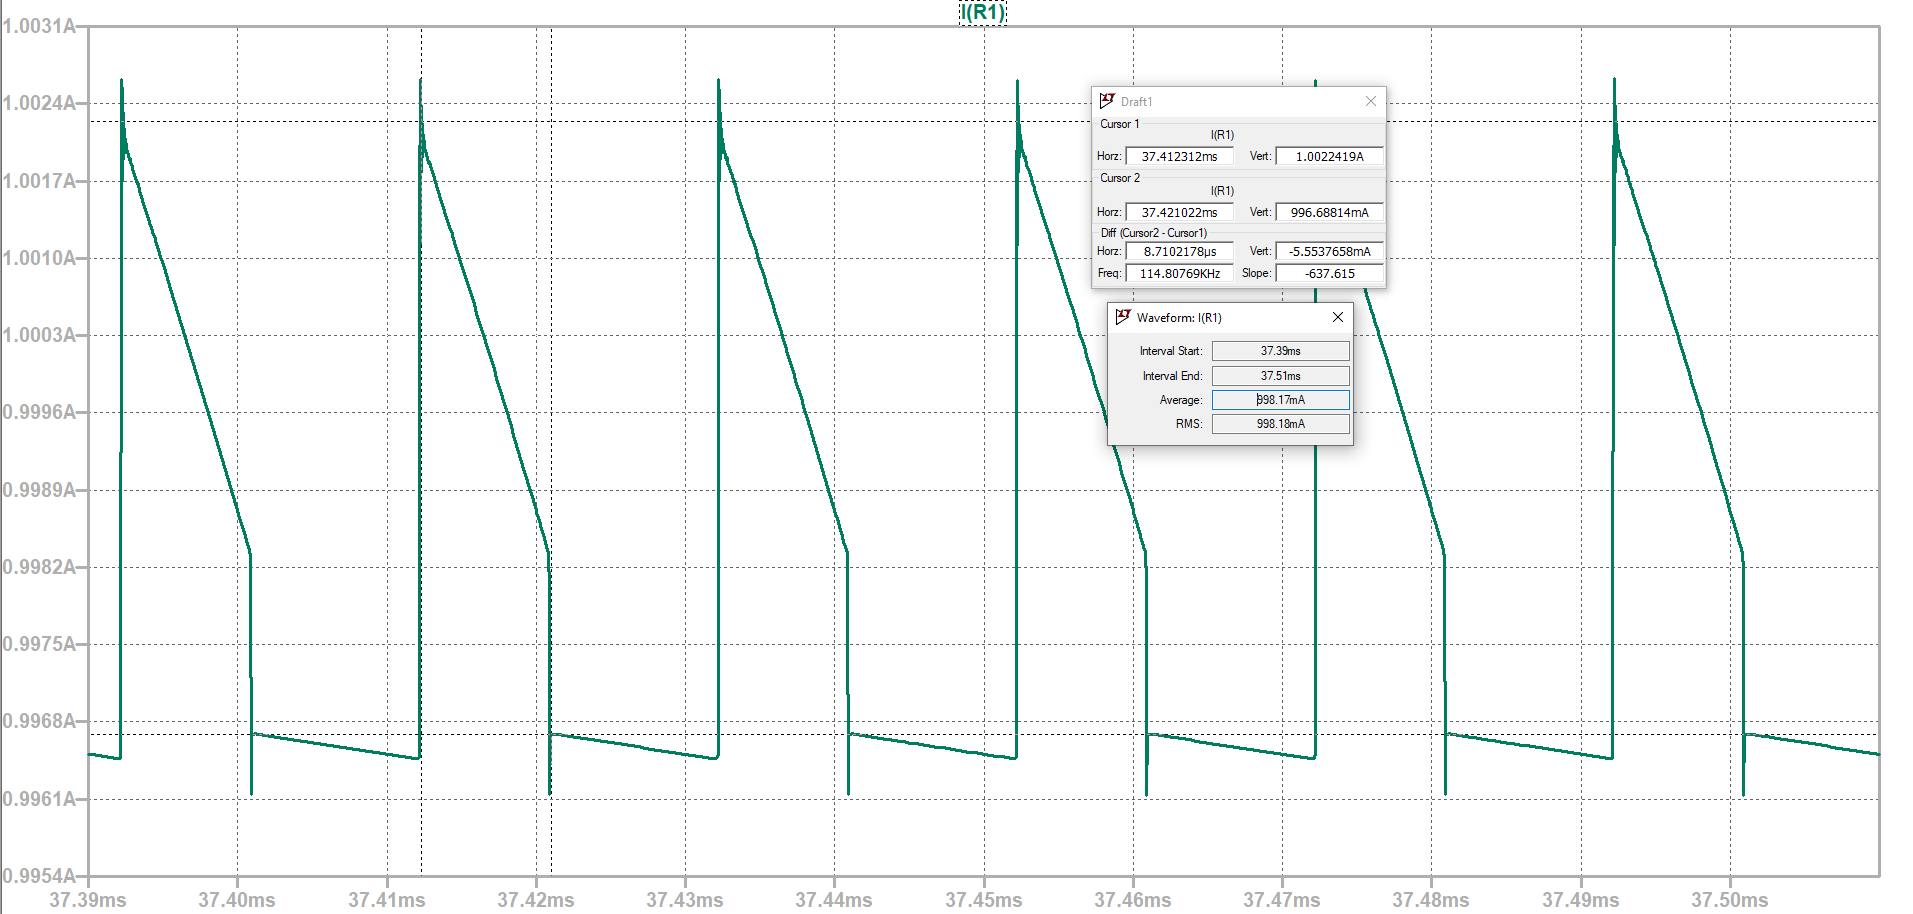
\includegraphics[width=0.6\textwidth]{Figures/iot-avg-ripple.png}
    \caption{$I_{out}$ waveform with parasitic included.}
    \label{fig:i_out}
\end{figure}
\begin{figure}[H]
    \centering
    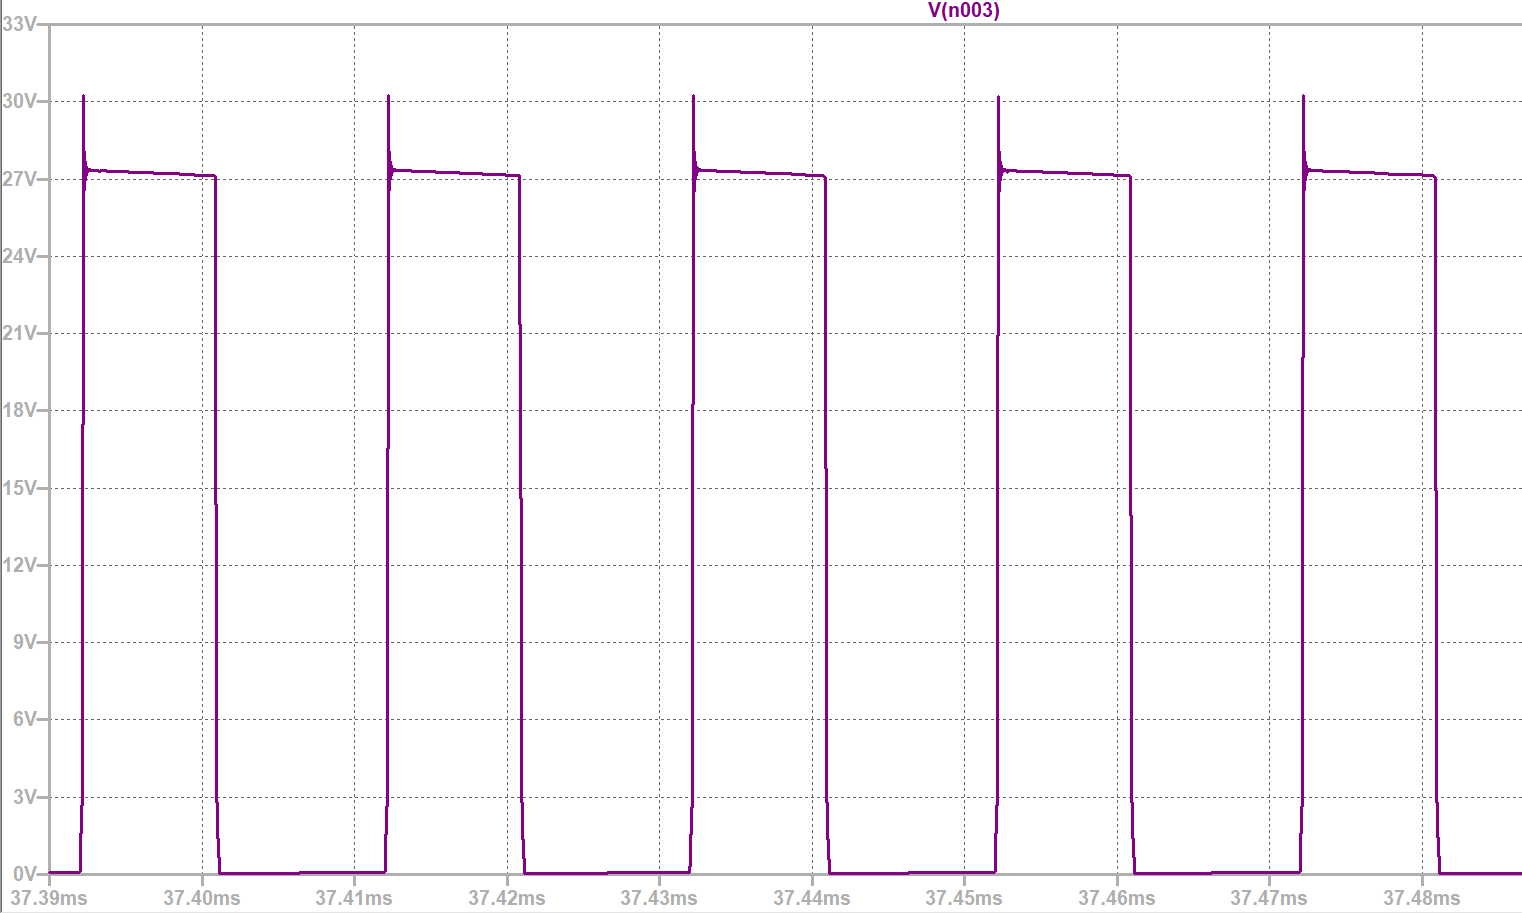
\includegraphics[width=0.6\textwidth]{Figures/mosfet-voltage.png}
    \caption{$V_{Q_1}$ waveform with parasitic included.}
    \label{fig:v_sw}
\end{figure}
\begin{figure}[H]
    \centering
    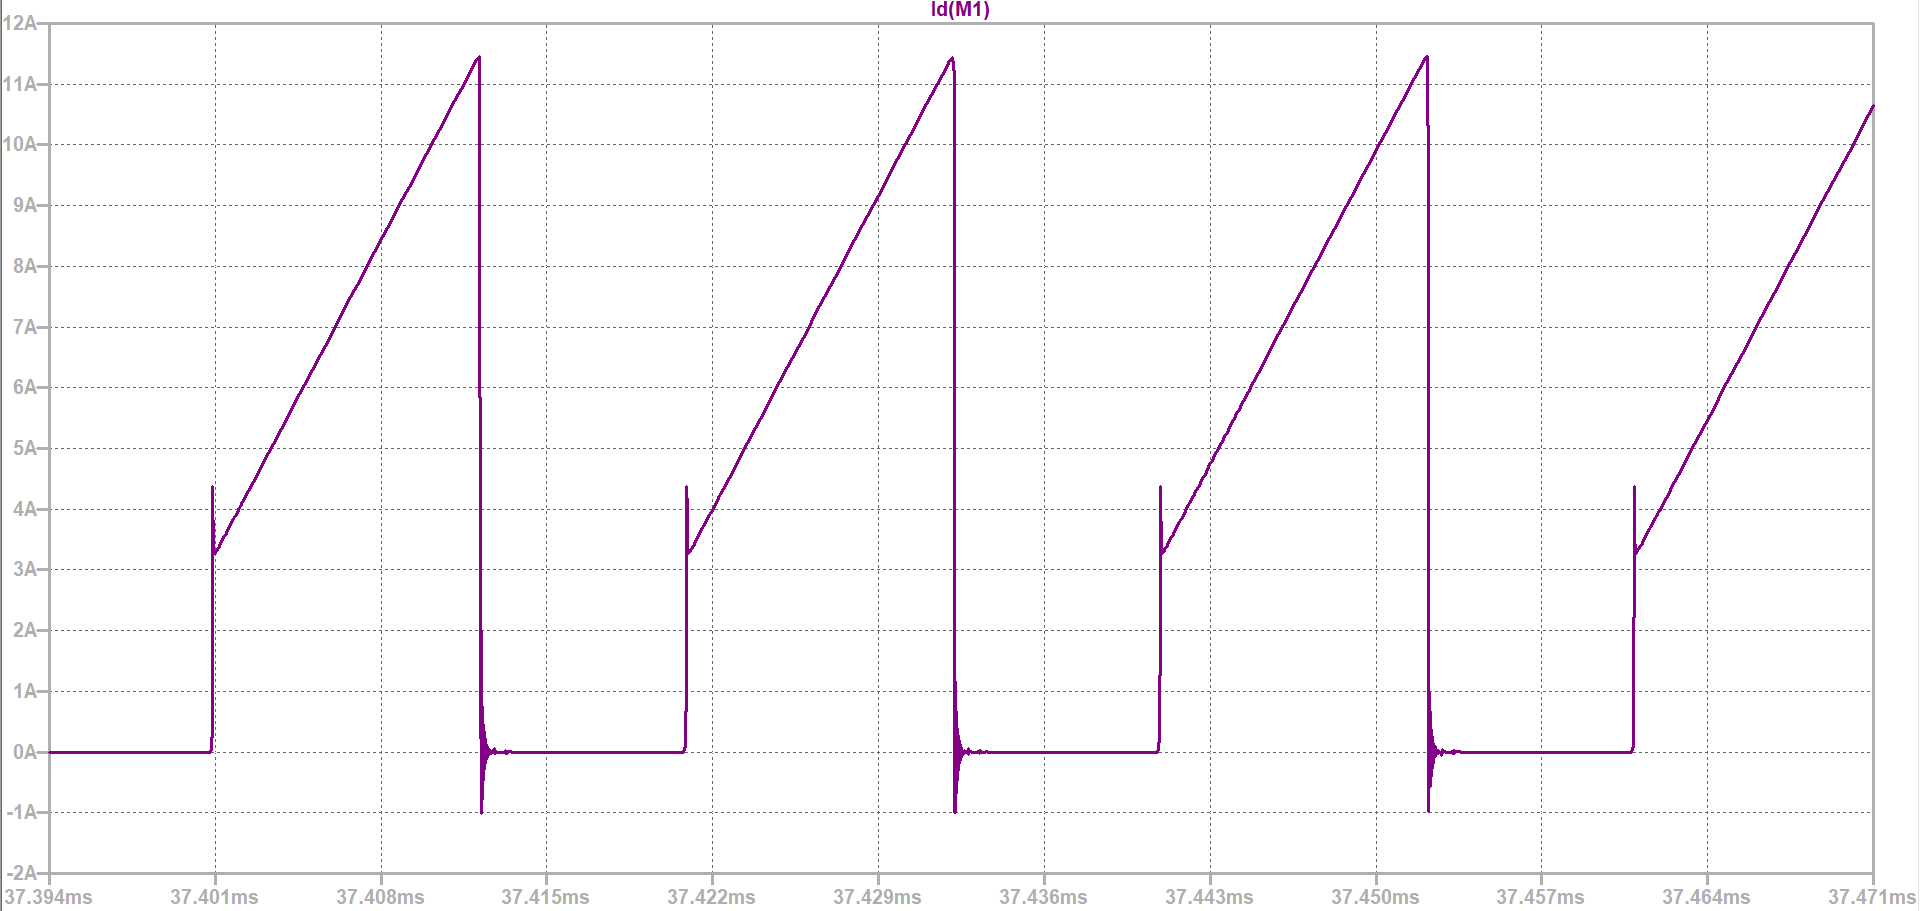
\includegraphics[width=0.6\textwidth]{Figures/mosfet-current.png}
    \caption{$I_{Q_1}$ waveform with parasitic included.}
    \label{fig:i_sw}
\end{figure}
\begin{figure}[H]
    \centering
    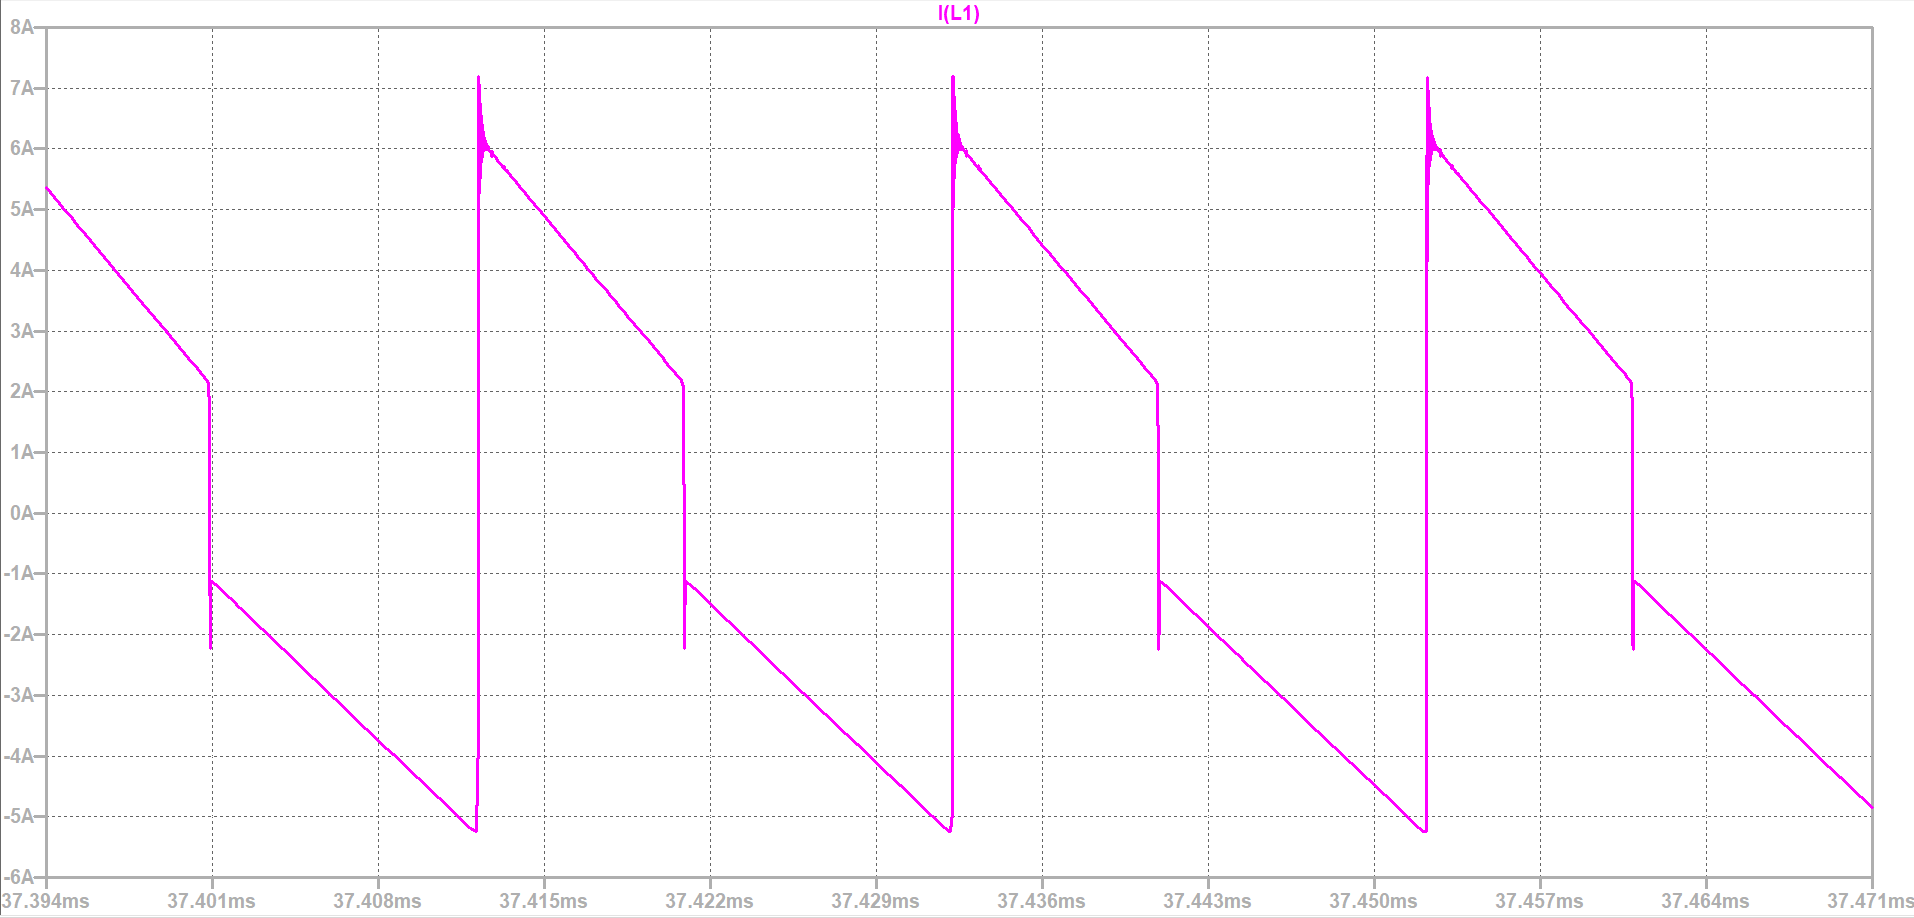
\includegraphics[width=0.6\textwidth]{Figures/trans_prim_curr.png}
    \caption{Caption}
    \label{fig:lm}
\end{figure}
\begin{figure}[H]
    \centering
    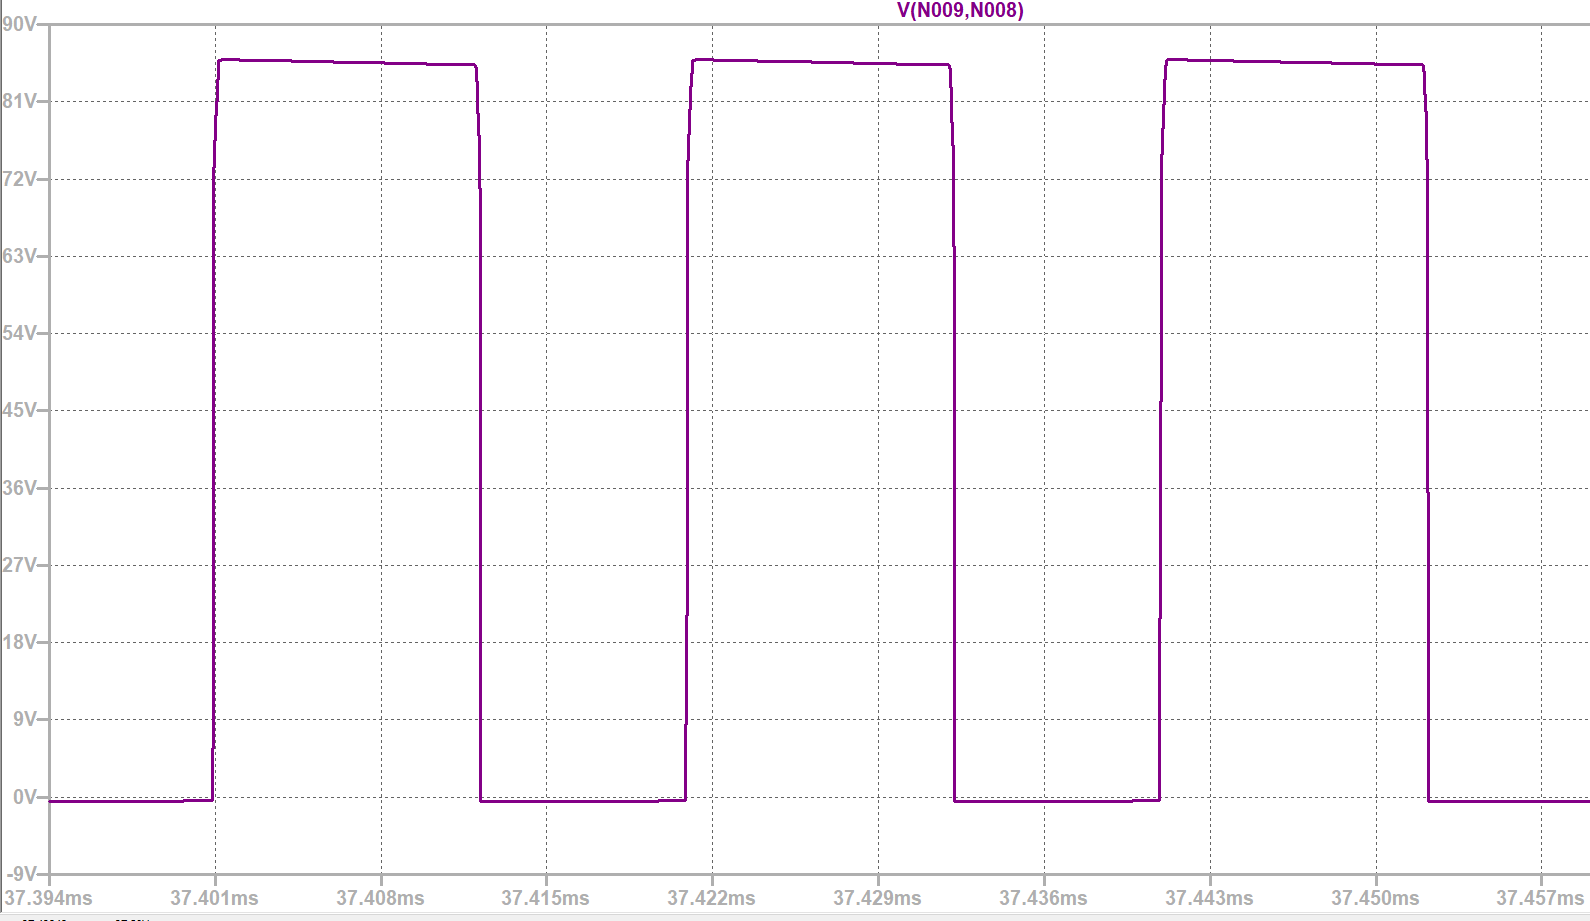
\includegraphics[width=0.6\textwidth]{Figures/diode-voltage.png}
    \caption{$V_{D_1}$ waveform with parasitic included.}
    \label{fig:v_d}
\end{figure}
\begin{figure}[H]
    \centering
    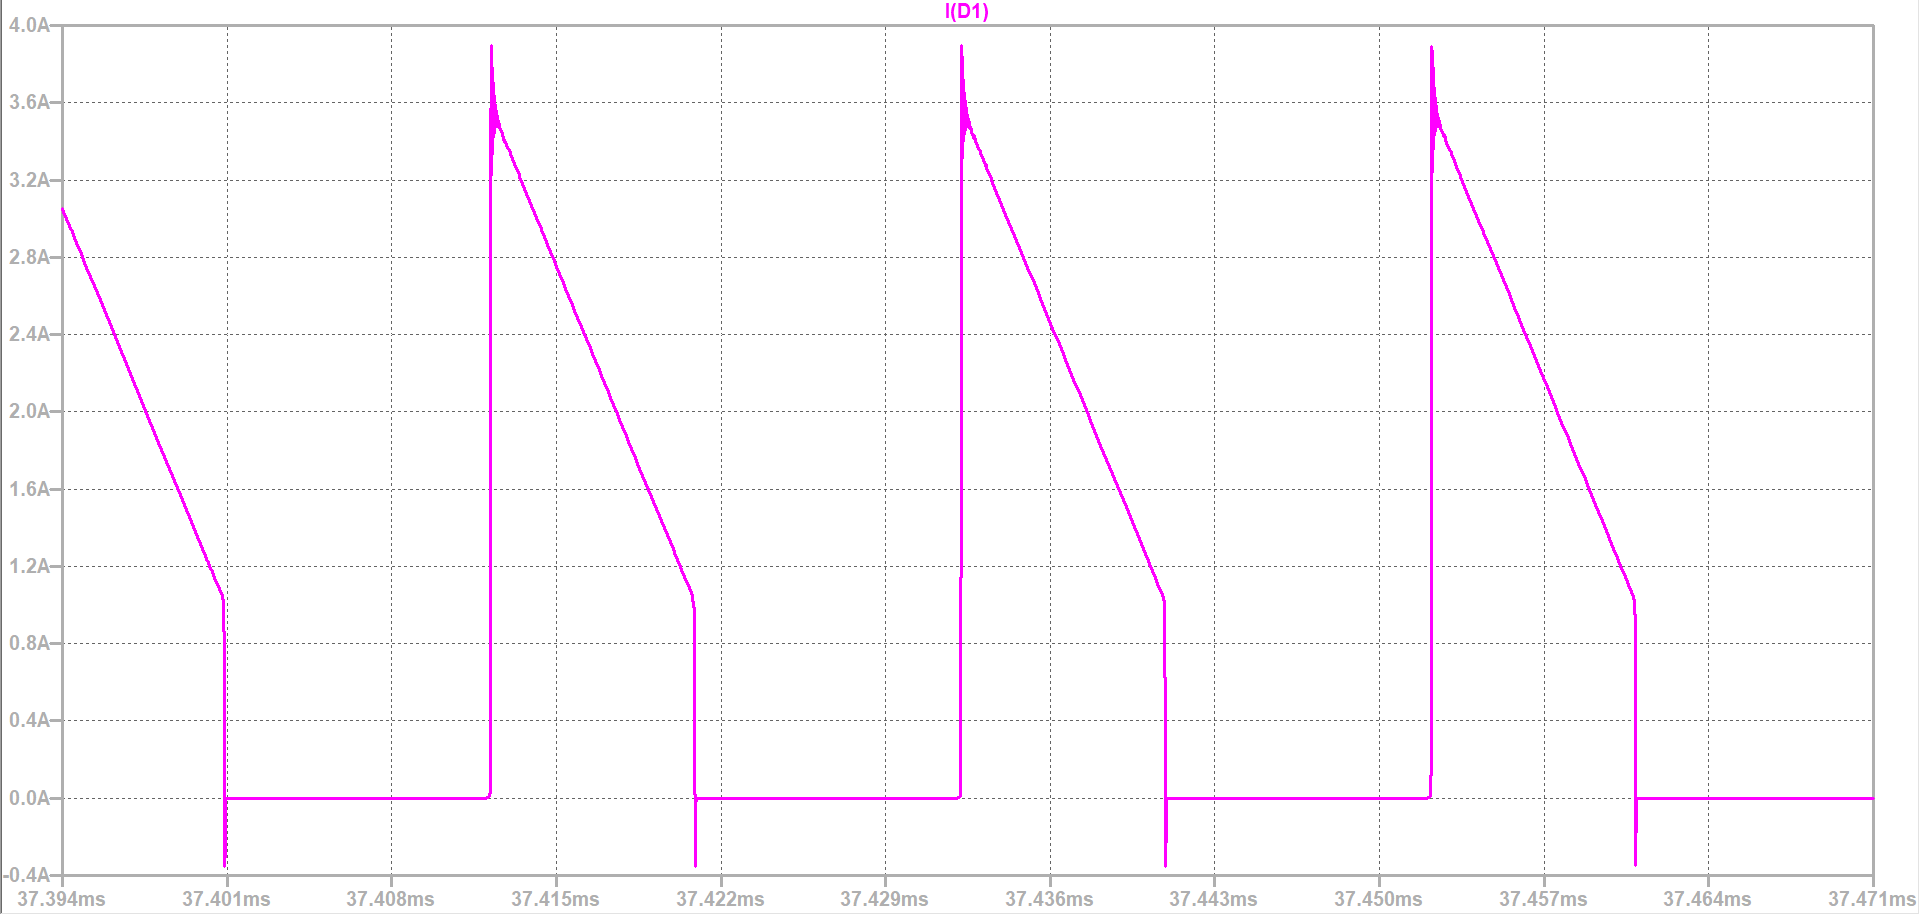
\includegraphics[width=0.6\textwidth]{Figures/diode-current.png}
    \caption{$I_{D_1}$ waveform with parasitic included.}
    \label{fig:i_d}
\end{figure}